\chapter{要素技術}
本章では,本研究で用いた深層学習に関連した要素技術と,ベースとする従来手法について述べる.

\section{Deep learning}
Deep learningは近年,自然言語処理など様々な分野で利用されている.
人間の脳におけるニューロンの構造を数理モデル(パーセプトロン)を用いて再現したニューラルネットワークを多層構造にすることで,
複雑なタスクの解決に必要な関数の表現力を高めたものである.
一般的な構造をFig. \ref{fig::network}示す.

\begin{figure}[h]
    \centering
    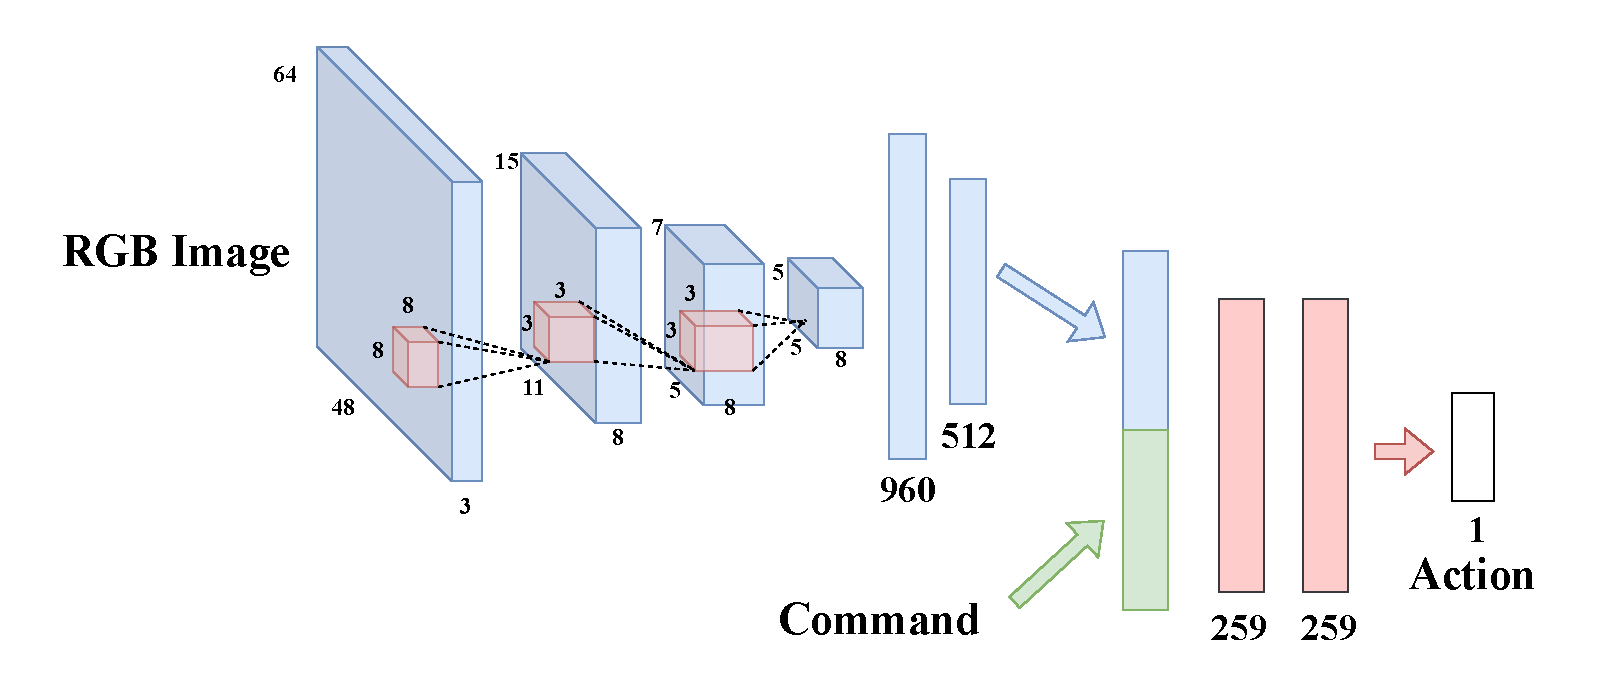
\includegraphics[width = 12cm]{./figs/network.pdf}
    \caption{Neual network}
    \label{fig::network}
\end{figure}

\section{end-to-end学習}
end-to-endとは,
Fig. \ref{fig::e2e}に示すように生データ(入力)から目的の結果(出力)を得るために必要な多段階の処理をNeusal Networkを用いて直接学習を行うものである.

実世界における自動運転を例に述べる.
人物や障害物などの物体認識,走行レーンの検出,経路計画,ステアリング制御
などの人間が設定した複数個のタスクを解く必要があるが,end-to-end学習では先程のタスクを人間が直接設定せずに
カメラ画像をニューラルネットワークに入力することで直接ステアリング操作を学習する.

\vspace{2.0zh}
\begin{figure}[h]
    \centering
    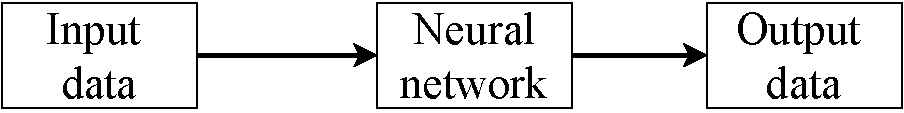
\includegraphics[width = 10cm]{./figs/e2e.pdf}
    \caption{Structure of end-to-end learning}
    \label{fig::e2e}
\end{figure}

\newpage
\section{Convolition Neual Network}
畳み込みニューラルネットワーク(convolutional neural network:CNN)は
画像認識や音声認識などの多次元の配列で表される複雑なデータを扱う処理へ用いられているニューラルネットワークである.
次のような特徴をもつ層で構成されている.

\begin{enumerate}
    \item 畳み込み層:入力データへフィルタ(カーネル)を用いて畳み込み演算を行うことで,特徴を抽出した特徴マップを取得する
    \item プーリング層:Maxプーリングなどの演算を用いて特徴マップのダウンサンプリングを行う
    \item 全結合層:畳み込み層,プーリング層で行った特徴を抽出したデータを一つのノードに
                      集約を行い,分類などの結果の出力を行う
\end{enumerate}


Krizhevskら\cite{Imagenet}はFig. \ref{fig::alex}で示すような3つの畳み込み層(convolutional layer),2つのプーリング層(pooling layer)
および 3 つの全結合層(fully connected layer)から構成したネットワークを用いて,
120万の高解像度画像を1,000の異なるクラスに分類をエラー率15.3\%で達成し,画像分類コンペティションであるILSVRC(ImageNet Large Scale Visual Recognition Competition)2012
で優勝をおさめた

\vspace{2.0zh}

\begin{figure}[h]
    \centering
    \includegraphics[width = 11.5cm]{./figs/alex.pdf}
    \caption{Alex net from \cite{Imagenet}}
    \label{fig::alex}
\end{figure}

\newpage
\section{地図ベースの制御器}
    \label{seigyo}
    従来手法と提案手法において,教師信号として用いる地図ベースの制御器について述べる.
    % 概要をFig. \ref{fig::navigation}に示す.
    地図べースの制御器は,ROS Navigation\_stack\cite{navigation:online}へ目標の経由地点(waypoint)の指示を行うwaypoint\_navを組み合わせたものである.
    ROS navigation\_stackは\ref{fig::mapbase}に示すように,事前に作成した地図とLiDAR,オドメトリを
    用いて,地図上の自己位置推定をParticle\_Filterによって確率的に行う「amcl」.
    障害物認識などの局所的または地図全体の大域的なコスト計算と,
    その結果を用いて経路計画,それに従ったモータ指令を行う「move\_base」
    などのパッケージを統合した自律走行用のメタパッケージである.
    従来手法,提案手法ではモータ指令を並進速度と角速度にわけ,並進速度は一定としている.
    % コスト計算を行うlocal\_costmapと結果を利用して,局所的な経路計画を行うlocal\_planner.
    % 地図に対して全体のコスト計算を行うglobal\_costmap,その結果を利用して大域的な経路計画を行うglobal\_plannner.
    % 「move\_base」のパッケージを統合した自律移動用のメタパッケージである.
    % 上記のと目標地点(waypoint)の指示を行う「waypoint\_nav」を組み合せることで,
    % Fig. \ref{fig::mapbase}に示す経路計画を行い,それに従ったモータ指令を行う
    
    
    % \vspace{2.0zh}
    % \begin{figure}[H]
    %     \centering
    %     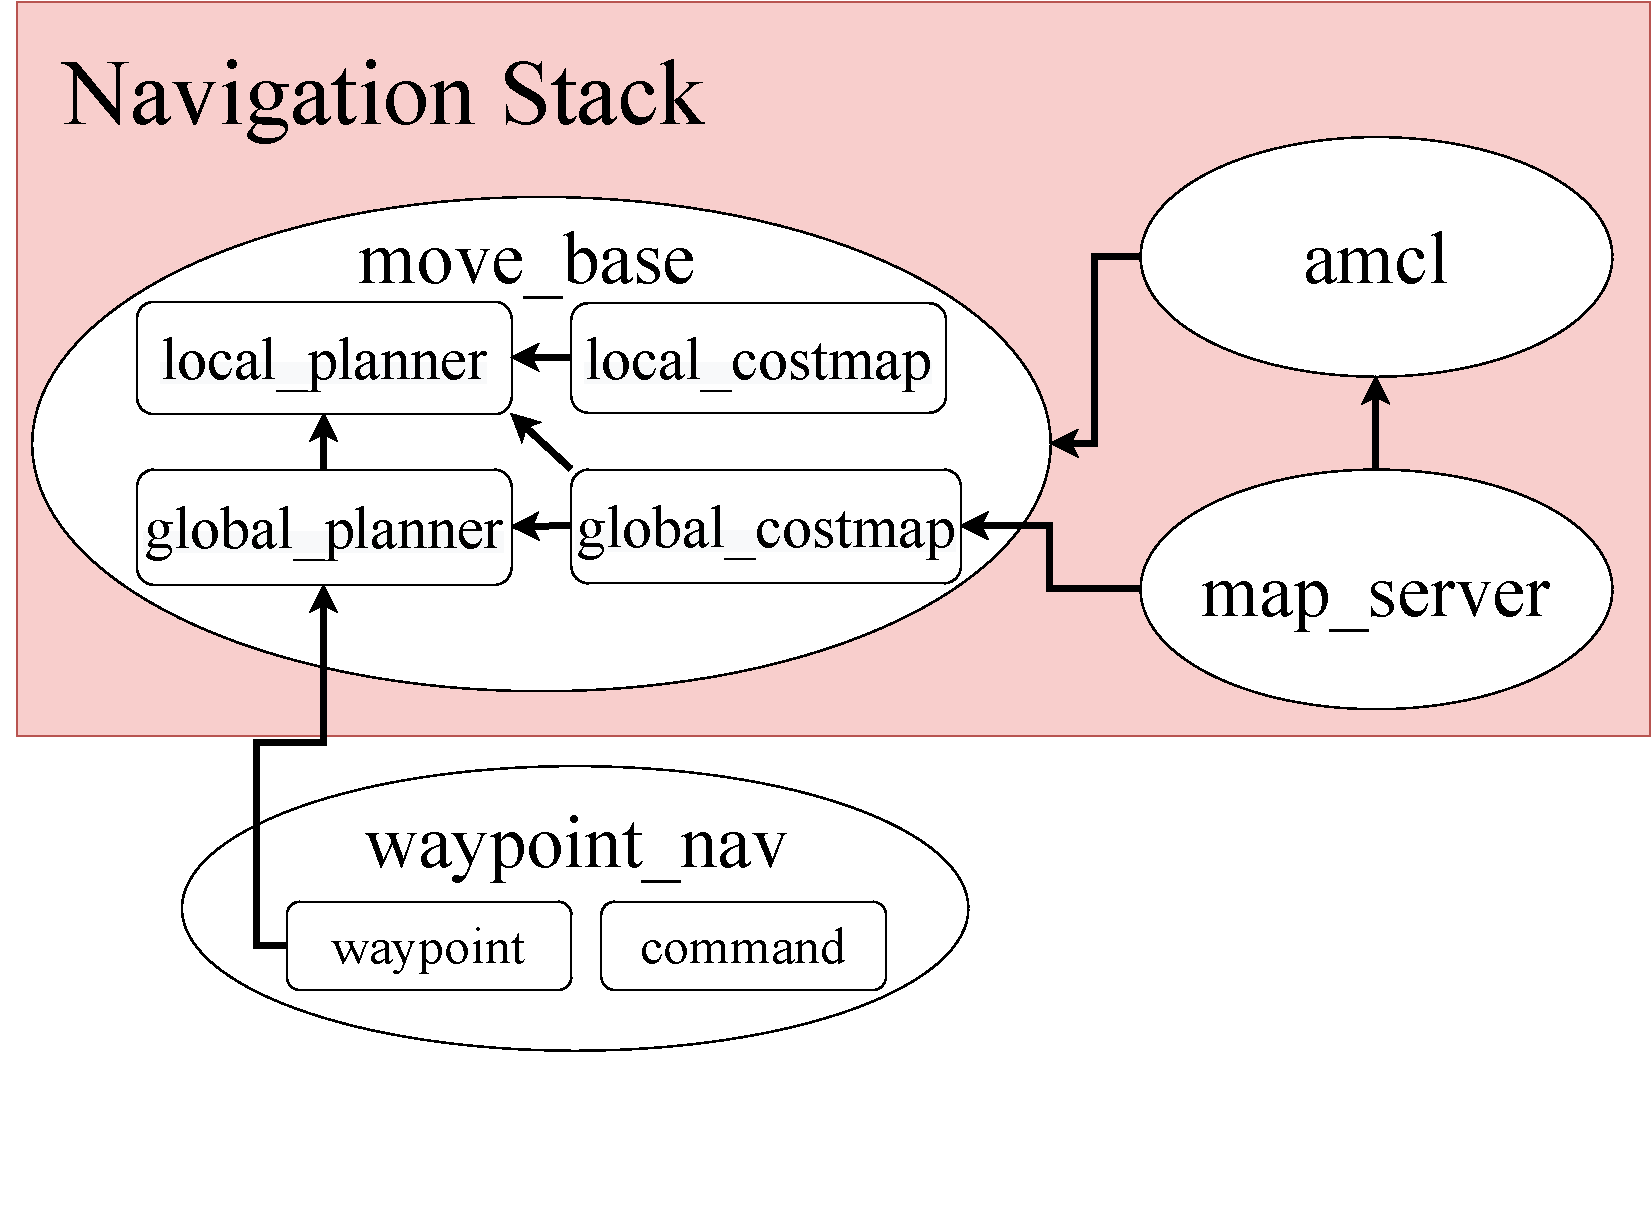
\includegraphics[width = 11cm]{./figs/navigation.pdf}
    %     \caption{Map-based controller}
    %     \label{fig::navigation}
    % \end{figure}

    \begin{figure}[H]
        \centering
        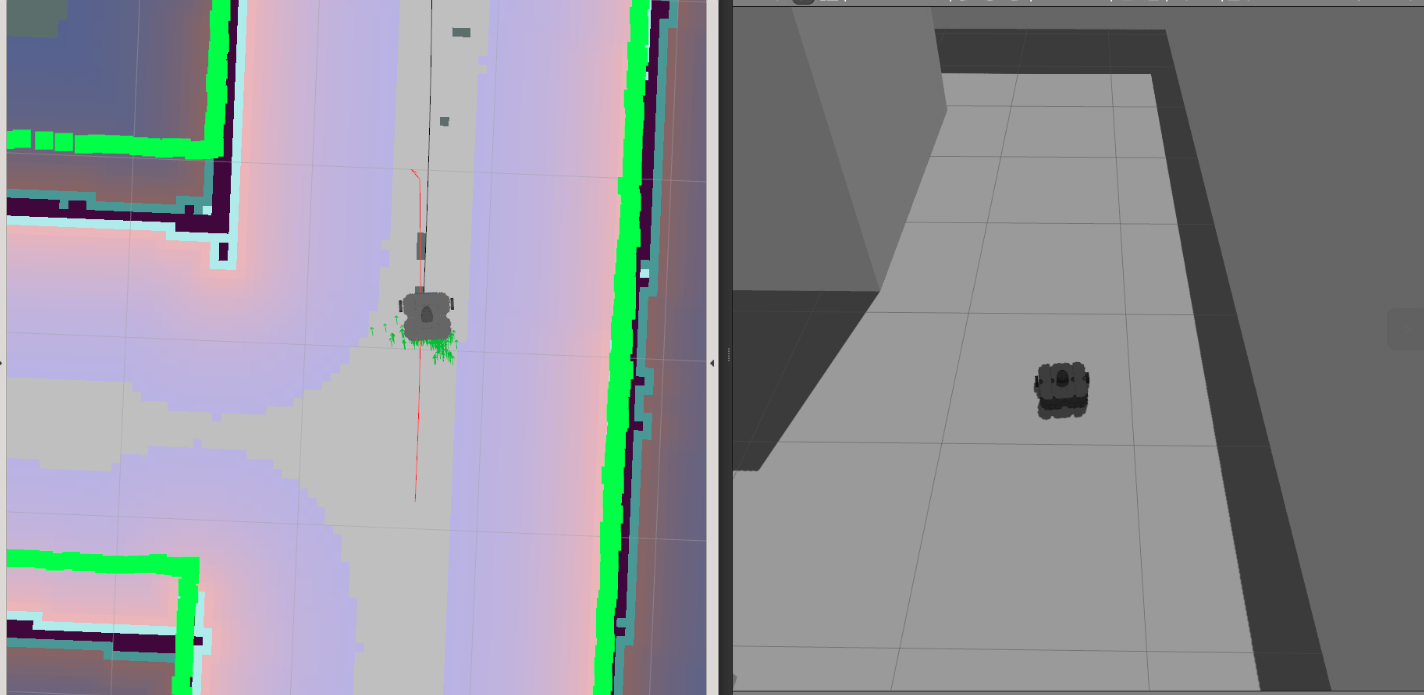
\includegraphics[width = 11cm]{./figs/mapbased.png}
        \caption{Map-based controller}
        \label{fig::mapbase}
    \end{figure}
\newpage
\section{従来手法}
本研究のベースとなる岡田らの研究について述べる.
先に述べたように,本論文では岡田らの手法を従来手法と呼ぶ.
従来手法は,LiDARを用いた走行を学習し,同じ行動を画像を用いて行う手法である.
学習器の訓練を行う「学習フェーズ」と,学習器の出力を用いて走行を行う「訓練フェーズ」の2つにわけられる.
なお,2つのフェーズでの並進速度は固定した同じ値を用いる.

学習フェーズをFig. \ref{fig::okada_method_ler}に示す.
LiDARとオドメトリを入力する地図ベースの制御器により自律移動を行い,それを
カメラ画像を用いて模倣する.
学習器は入力をカメラ画像,出力を自律走行時の角速度としてend-to-end学習を行う.
\begin{figure}[h]
    \centering
    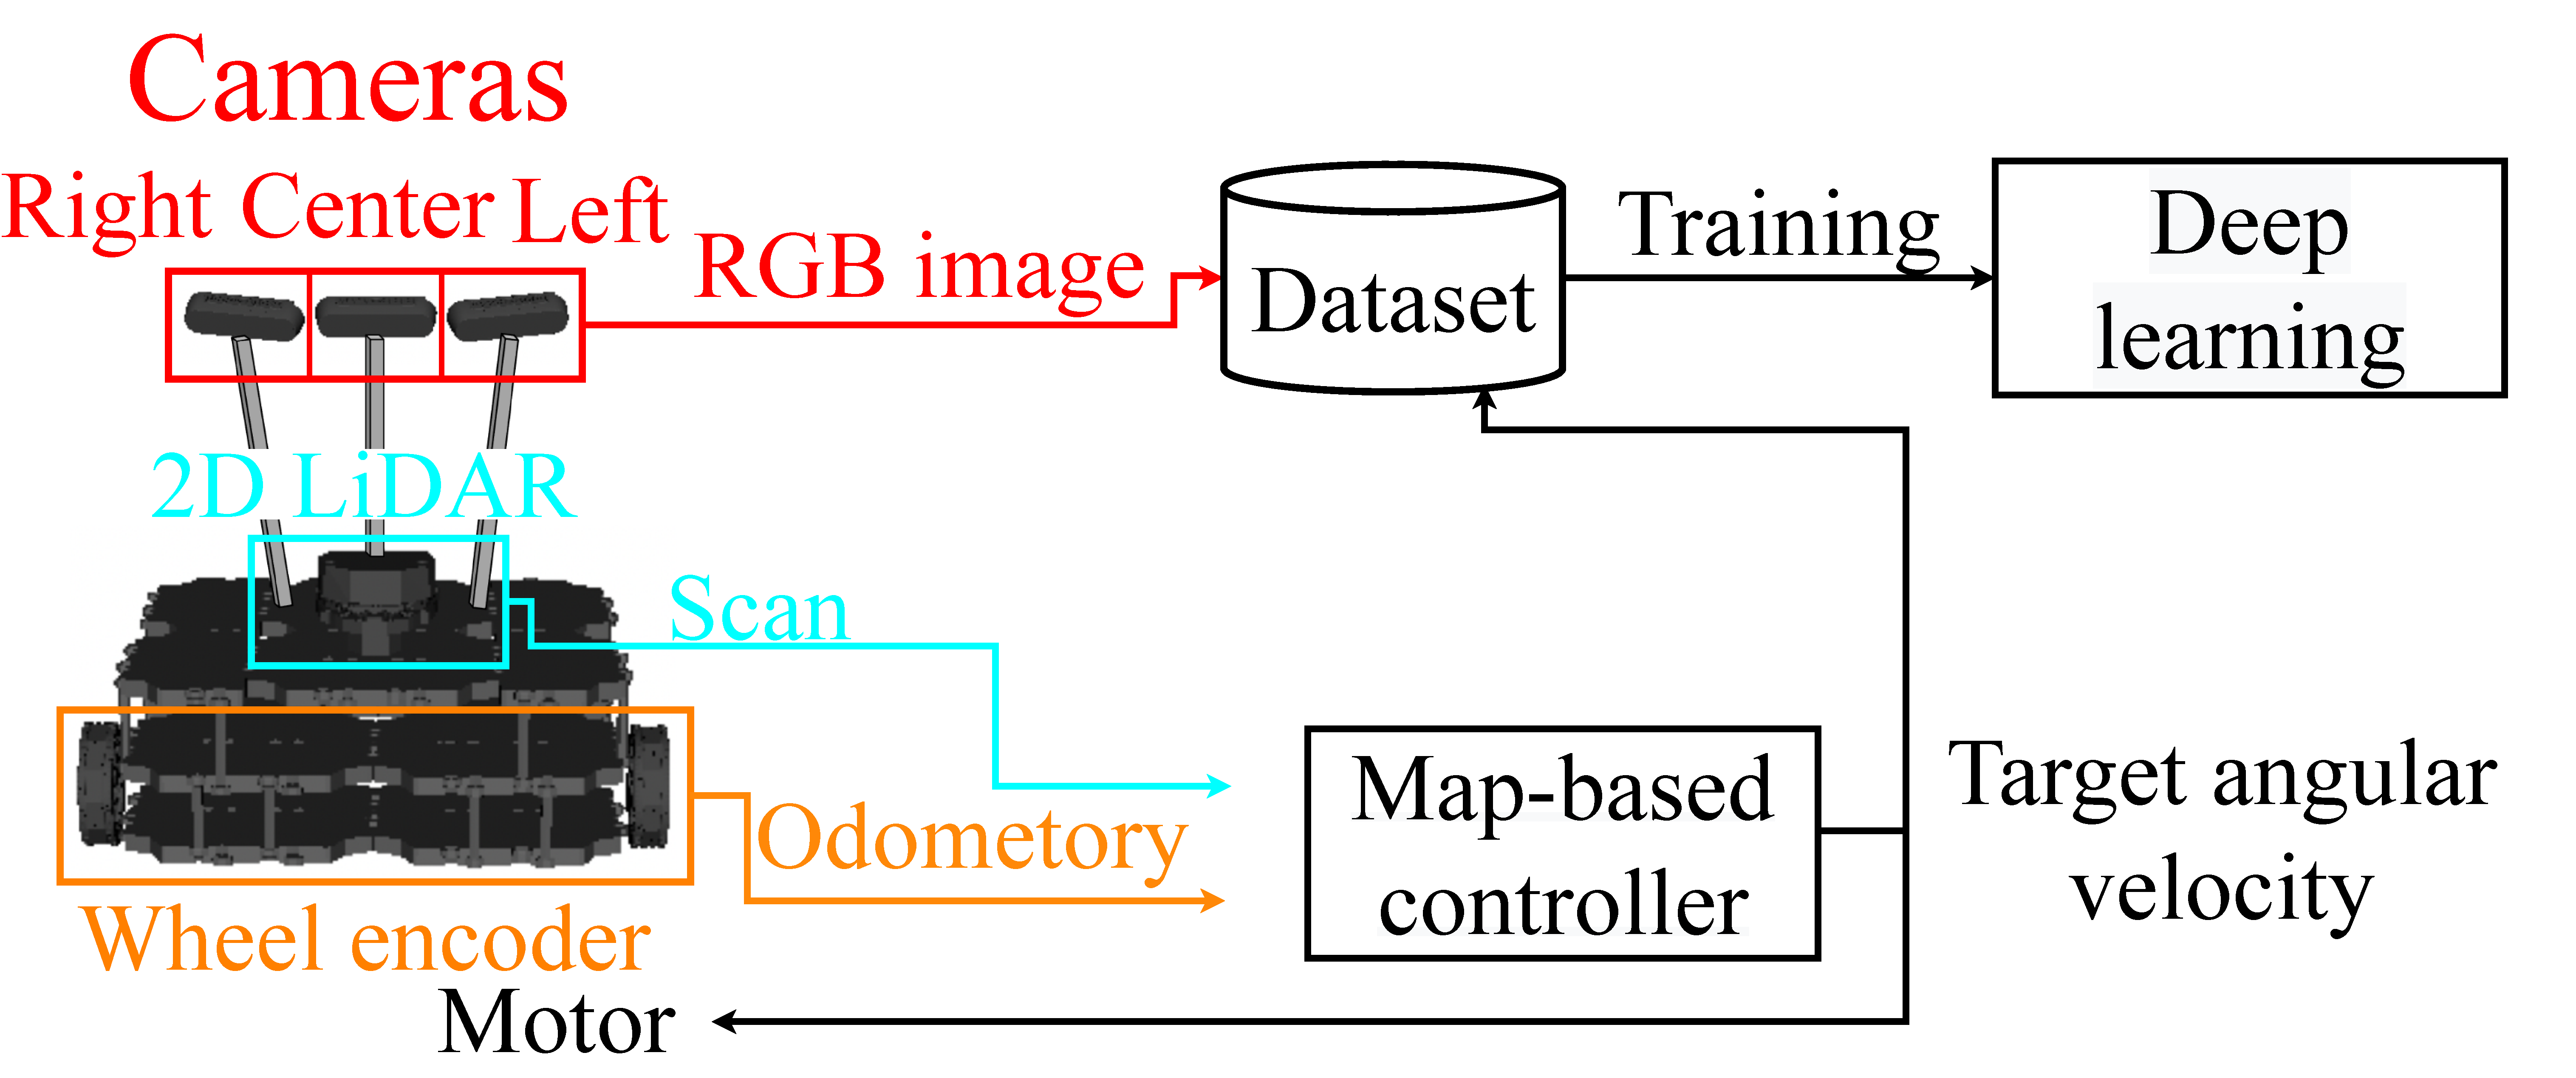
\includegraphics[width = 12cm]{./figs/system_learning_okada.pdf}
    \caption{Learning phase of conventional method}
    \label{fig::okada_method_ler}
\end{figure}

\newpage
学習フェーズでは機体の中央, 左,右に傾けて取り付けた3つのカメラを用いる.
その際,直進時に,同時に旋回の行動を取得すること及び過学習の抑制を目的として,
Table\ref{tb::camera_ang}に示すような処理を行う.
\begin{table}[H]
    \centering
    \caption{Angular velocity ofset}
    \begin{tabular}{|c|c|ll}
    \hline
    Left camera   & Angular velocity of Map-based controller + 0.2 rad/s \\ \hline
    Center camera & Angular velocity of Map-based controller             \\ \hline
    Right camera  & Angular velocity of Map-based controller - 0.2 rad/s  \\ \hline
    \end{tabular}
    \label{tb::camera_ang}
    \end{table}
また,Fig. \ref{fig::okada_path}に示すように実際にロボットを制御する行動と経路に沿う行動を別に扱うことで,
常に経路に沿う行動をデータセットに加えることを可能にしている.
\begin{figure}[h]
    \centering
    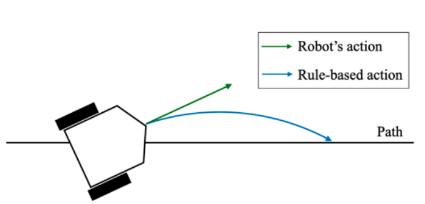
\includegraphics[width = 10cm]{./figs/okada_path.png}
    \caption{Collect the rule-based actions the robot's actions from \cite{okada}}
    \label{fig::okada_path}
\end{figure}

\newpage
学習器の訓練後,Fig. \ref{fig::okada_method_test}で示すテストフェーズへ移行する.
テストフェーズでは,カメラ画像を入力する学習器の出力する角速度を用いて自律走行を行う.
なお,テストフェーズでは中央のカメラのみを用いる.
\begin{figure}[h]
    \centering
    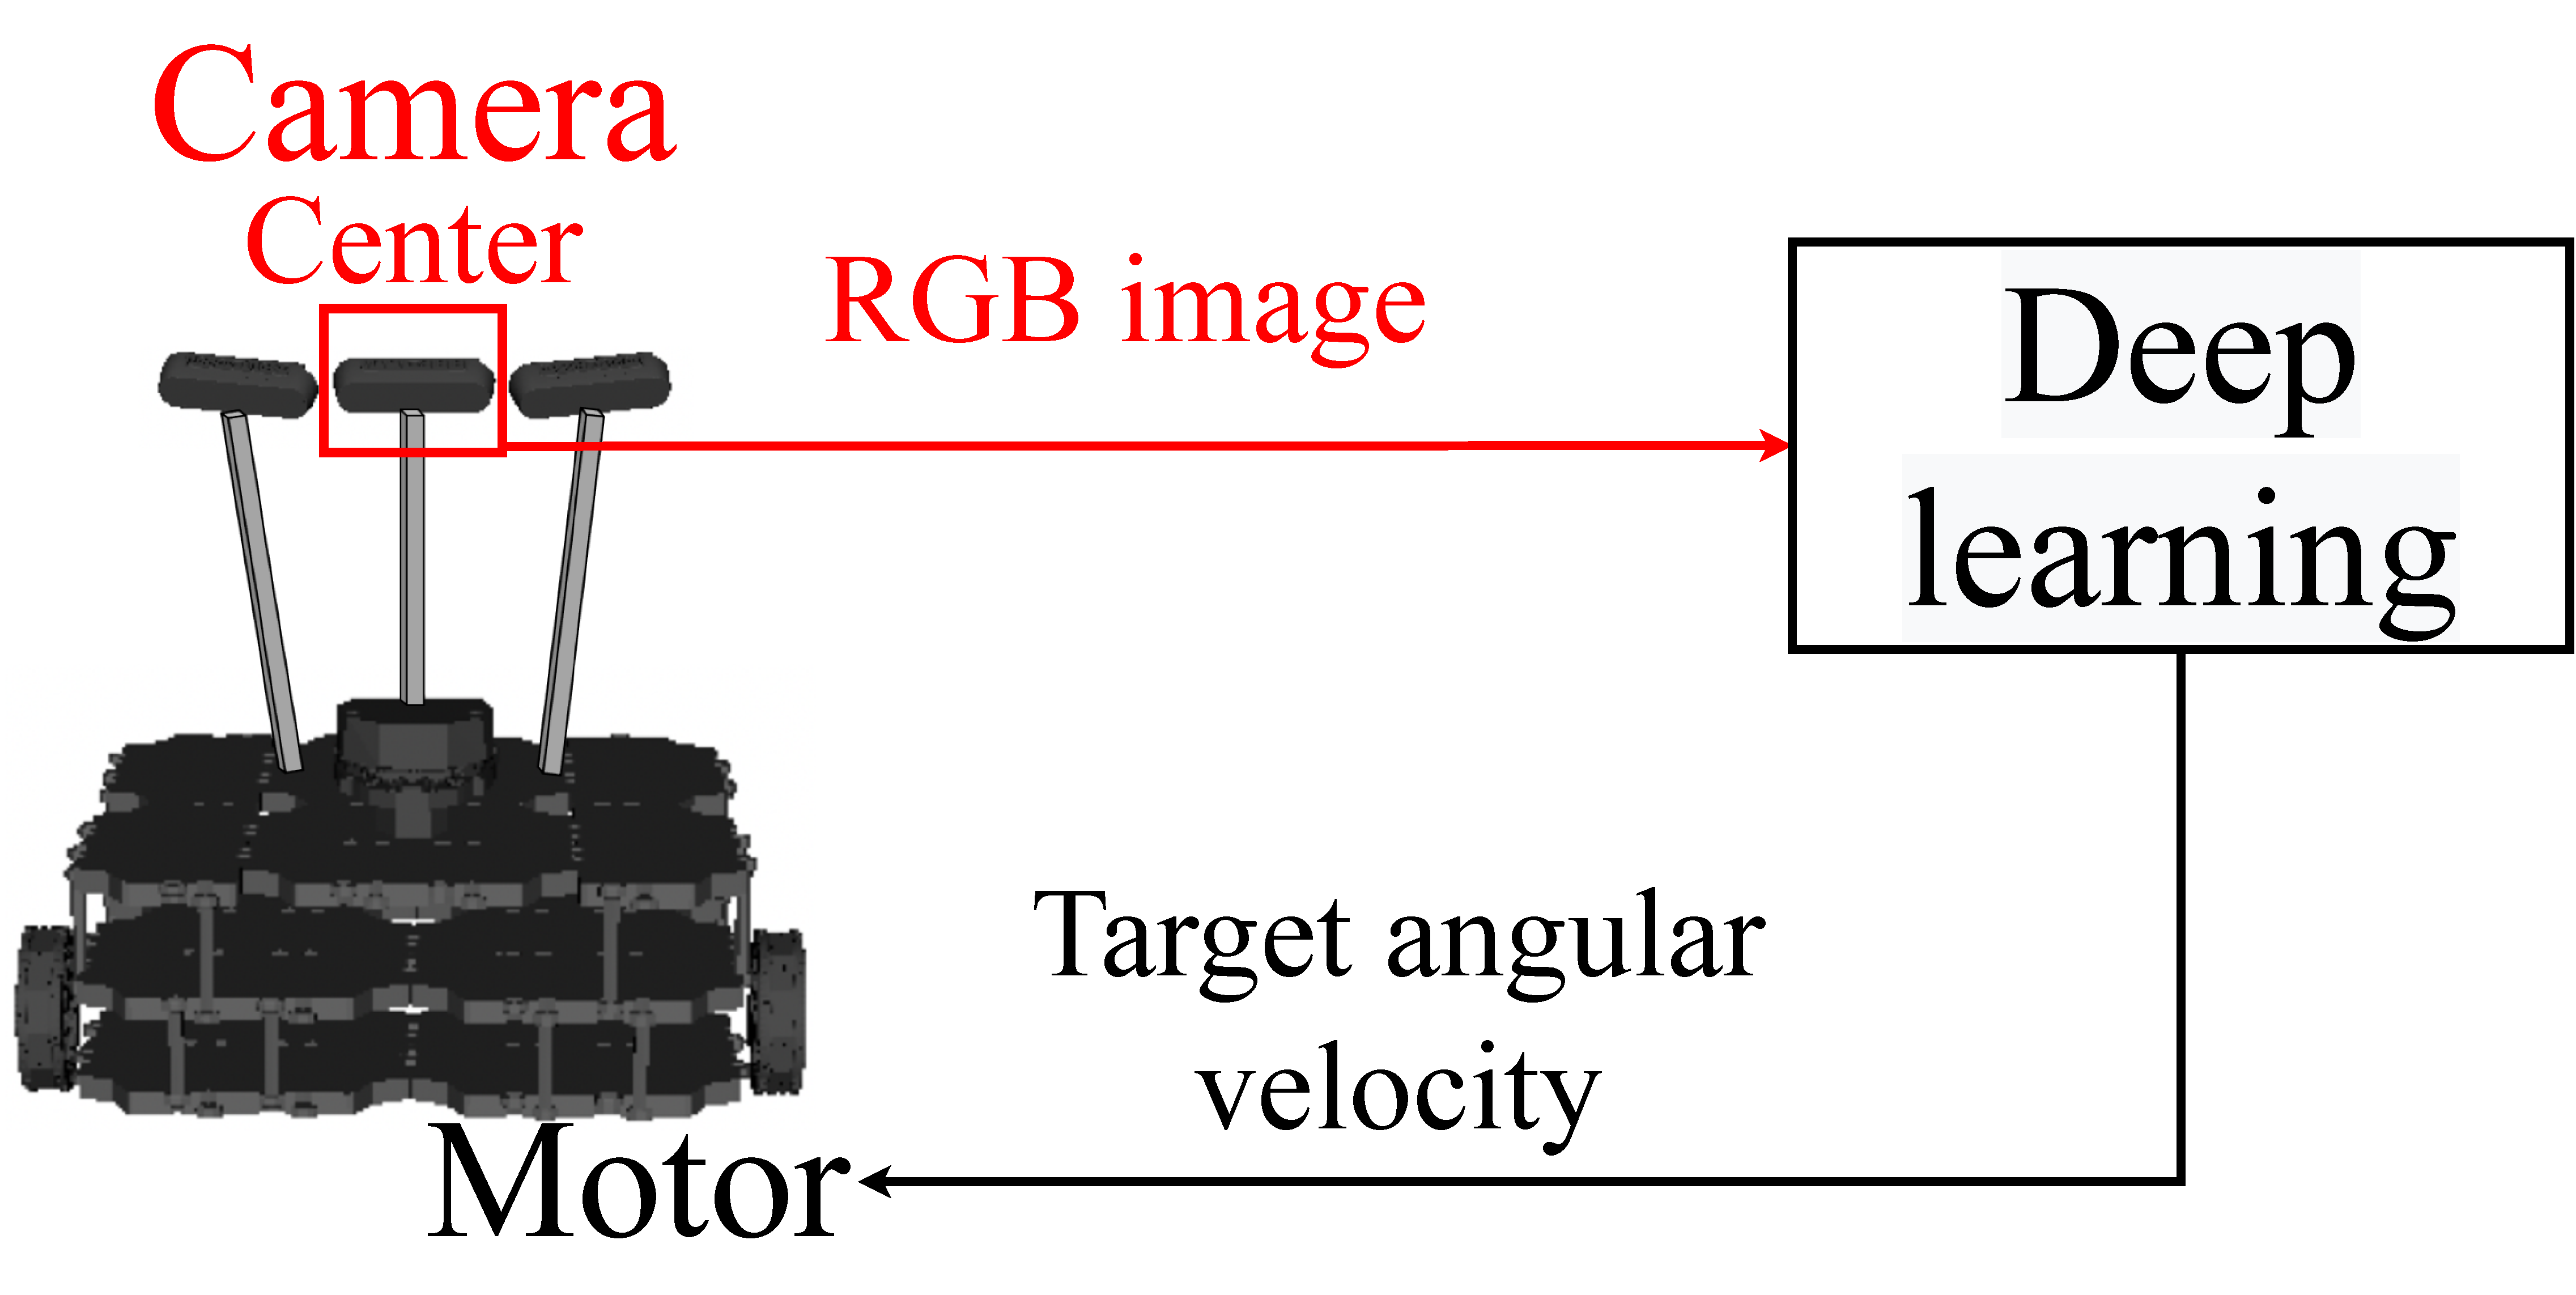
\includegraphics[width = 10cm]{./figs/okada_method_test.pdf}
    \caption{Test phase of conventional method}
    \label{fig::okada_method_test}
\end{figure}